%%% Fiktivní kapitola s ukázkami tabulek, obrázků a kódu

\chapter{Implementace projektu}
V předchozí kapitole jsme prošli funkční požadavky, očekávané od vyvíjeného
souboru programů. Následuje rozbor jednotlivých modulů, které vznikly při
vlastní implementaci. 

\paragraph{Programovací jazyk}
Celý projekt je napsána v programovacím jazyce \textbf{Python}. Cílem projektu
je vytvořit čitelnou rozšířitelnou platformu, která bude uživateli jednoduše
dostupná. Pokud uživatel bude mít potřebu vytvořené moduly jakkoli měnit nebo
rozšiřovat, Python toto bez problémů umožní. Jednoduchá čitelnost Pythonu
spojená s rychlostí, jakou mohou být prováděny iterace změn, bez potřeby
zdlouhavého překladu celé knihovny, se nám zdají býti dostatečně užitečné
vlastnosti volbu Pythonu jako jazyka pro tento projekt.

\paragraph{Struktura projektu}

%TODO: Change basic imp_graph
\begin{figure}[!htb]
    \centering
    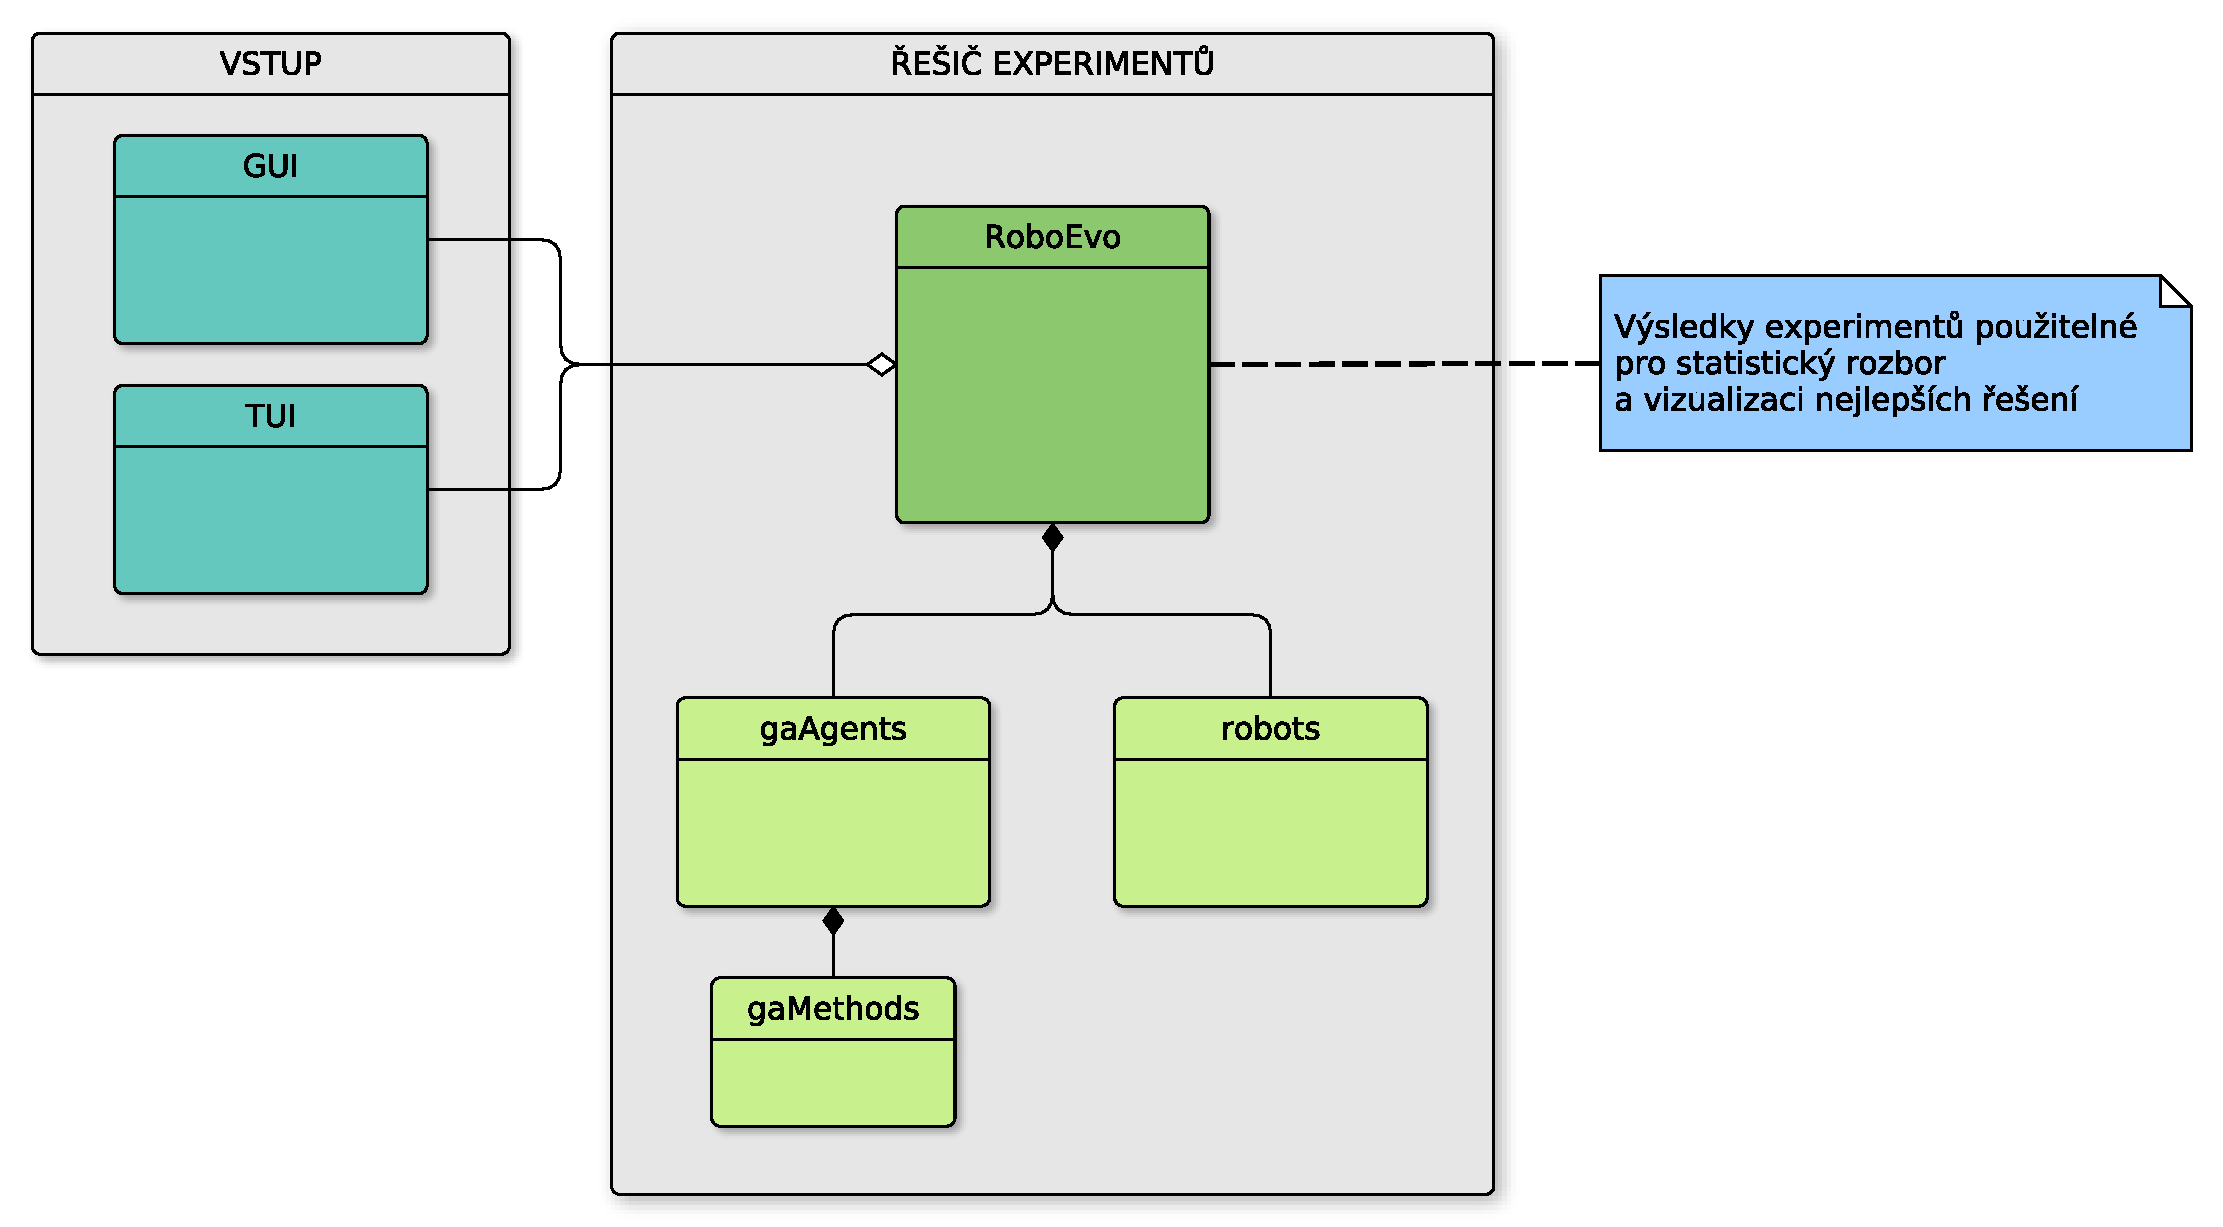
\includegraphics[width=1\textwidth]{../img/BP_imp_graph.pdf}
    \caption{Struktura projektu}
    \label{fig:struktura}
\end{figure}

Obrázek \ref{fig:struktura} popisuje na jaké části je projekt rozdělen.
Centrální částí je modul \emph{RoboEvo}, pomocí kterého knihovna provádí
evoluční experimenty. Tento modul se pro přehlednost a rozšířitelnost kódu
skládá z několika menších částí -- \emph{gaAgents} (popisující agenty a vlastní
genetické operátory) a \emph{robots} (udržující jednotný způsob přístupu k
různým robotům). 

Jak popisují funkční požadavky (v sekci \ref{Specifikace-funkčnípožadavky}),
projekt umožňuje několik možných způsobů práce s naší knihovny. Dva základní
možné přístupy jsou za pomoci grafického, nebo textového rozhraní. Tyto
přístupy jsou v projektu rozděleny do \emph{GUI} (\emph{Graphical User
Interface}) a \emph{TUI} (\emph{Text-based User Interface}) modulů. Uživatel,
který bude chtít pracovat s kódem části knihovny zaměřené na vytváření a
provádění experimentů s evolučním vývojem, se dále může zaměřit na hlavní modul
\emph{RoboEvo} (a s ním spojené pomocné moduly).

\paragraph{} 
Dále v této kapitole v sekci \ref{imp:roboevo} popíšeme centrální modul
\emph{RoboEvo} pracující s několika dalšími pomocnými moduly, jejichž
implementace popíšeme v dalších oddílech. Popíšeme třídu agentů v oddílu
\ref{imp:gaAgents}. Implementace vlastních genetických operátorů se nachází v
oddílu \ref{imp:gaMethods}. Vlastní třída \emph{robots} propojující roboty ze
simulátoru \emph{MuJoCo} (MuJoCo popsáno v základních pojmech v oddílu
\ref{MuJoCo}) s ostatními třídami je vysvětlena (v oddílu \ref{imp:robots}).
Následně si moduly umožňující uživateli práci s knihovnou buď pomocí grafického
prostředí (v sekci \ref{imp:GUI}), nebo pomocí příkazové řádky (v sekci
\ref{imp:TUI}). Jako poslední (v sekci \ref{imp:experimentsetter}) si
představíme implementaci třídy \emph{experimentSetter}, sloužící k uchování a
předvolbě parametrů pro experimenty a usnadňující tak provádění většího
množství experimentů.

\section{RoboEvo a pomocné moduly}
V této sekci popíšeme hlavní modul \emph{RoboEvo} a jeho pomocné moduly\\
\emph{gaAgents}, \emph{gaMethods} a \emph{robots}. Soubor těchto modulů tvoří
hlavní část celého projektu, obsahující celý proces umožňující provádění
evolučních experimentů s roboty. Vybrané rozdělení modulů bylo vytvořeno pro
zjednodušení čitelnosti a rozšířitelnosti kódu, kde nyní každý modul
zprostředkovává velmi specifickou roli v procesu evolučního vývoje, a tudíž je
pro uživatele jednoduché tyto části upravovat. Tato část projektu je zároveň
zcela oddělena od zpracování uživatelského vstupu, který do hlavního modulu
vstupuje z vnějších modulů, až ve chvíli zahájení experimentu. 

\subsection{Modul RoboEvo} \label{imp:roboevo}
Modul \emph{RoboEvo} je centrální modul tohoto projektu, sloužící pro spouštění
a běh experimentů s evolučním vývojem robotů. 

Každý experiment se skládá z několika nezávislých částí. Experiment může
využívat různé typy evolučních agentů s různými genetickými operátory a může se
snažit vyvíjet různé typy robotů. Jak bylo zmíněno výše, tyto částí jsou pro
přehlednost, čitelnost a rozšířitelnost kódu oddělené do vlastních menších
implementací, rozšiřující hlavní modul (jednotlivé implementace budou popsány v
dalších oddílech). 

\paragraph{Implementace modulu \emph{RoboEvo}}
Tento modul obsahuje funkce sloužící jak k inicializaci evolučních experimentů,
tak k samotnému běhu evolučních algoritmů, včetně propojení s knihovnou
\emph{Gymnasium} od Farama Foundation (popsáno v sekci \ref{Simulátory -
Porovnání}), zprostředkovávající simulaci fyzikálního prostředí pro testování
jedinců.

Hlavní funkcí, která z vnějšího vstupního prostředí (např. \emph{GUI},
\emph{TUI}, vlastní modul uživatele) přijímá parametry pro spuštění
experimentů, je funkce \linebreak\texttt{run\_experiment}. Povinným parametrem
této funkce jsou parametry \linebreak experimentu, které jsou pro zapouzdření
vloženy do jednoduché třídy \linebreak\texttt{ExperimentParams} (modul
\emph{experiment\_params}) obsahující následující hodnoty:

%TODO: LOOK AT BLACK BARS FOR LINEBREAKS \linebreak

%TODO: care for params changes - show graph (possibly)
\begin{itemize}
    \item \texttt{robot} -- zvolený robot z modulu \texttt{robots},
    \item \texttt{agent} -- zvolený agenta z modulu \texttt{gaAgents},
    \item \texttt{ga\_population\_size} -- velikost populace jedinců v
        evolučním algoritmu,
    \item \texttt{ga\_generation\_count} -- počet generací, po které bude
        evoluční algoritmus běžet,
    \item \texttt{show\_best} -- příznak určující, zda po doběhnutí evolučního
        algoritmu \\chceme v simulovaném prostředí zobrazit řešení nejlepšího
        jedince,
    \item \texttt{save\_best} -- příznak určující, zda po doběhnutí evolučního
        algoritmu \\chceme uložit nejlepšího jedince,
    \item \texttt{save\_dir} -- cesta ke složce, kam chceme uložit data z běhu
        evolučního algoritmu (pokud neexistuje, je složka automaticky vytvořena
        po doběhnutí algoritmu),
    \item \texttt{note} -- případná poznámka, kterou může uživatel speciálně
        odlišit název dat, ukládaných po doběhnutí algoritmu.
\end{itemize}

Funkce \texttt{run\_experiment} zpracovává tyto parametry a zajišťuje vše
potřebné pro běh experimentu. V přípravě probíhá spouštění výpočetních
jednotek pro paralelizaci testovacího prostředí (umožňující ohodnocení
populace jedinců paralelně). Následně proběhne spuštění evolučního algoritmu se
zvolenými parametry, po kterém funkce uloží data vygenerovaná evolučním
algoritmem -- fitness hodnoty jedinců v každé generaci, celá
populace jedinců z poslední generace a (volitelné) nejlepší řešení na konci
experimentu. Tato data jsou uložená do složky, dostupné na cestě popsané v
\texttt{save\_dir} parametru.

% \pagebreak
% Těmito parametry jsou:
% \begin{itemize}
    % \item \texttt{-{}-experiment} -- argument přijímající textový vstup
    %     specifikující jméno experimentu, jehož parametry chceme načíst a
    %     spustit (pracující s modulem \texttt{experiment\_setter} popsaného v
    %     oddíle \ref{imp:experimentsetter}),
    % \item \texttt{-{}-experiment\_names} -- při výběru tohoto argumentu při
    %     spuštění programu program vypíše názvy všech dostupných vytvořených
    %     experimentů z modulu \texttt{experiment\_setter} a následně se ukončí,
    % \item \texttt{-{}-batch} -- argument přijímající číselnou hodnotu,
    %     specifikující kolikrát se má nakonfigurovaný experiment opakovaně
    %     spustit (používané pro statistické vyhodnocení výsledků experimentů),
    % \item \texttt{-{}-batch\_note} -- textový argument umožňující připojit
    %     vlastní poznámku k názvu složky, do které se experimenty z
    %     několikanásobného spuštění ukládají (argument nemá žádný efekt pro
    %     experimenty z modulu \texttt{experiment\_setter}),
    % \item \texttt{-{}-open} -- textový argument přijímající cestu k uloženým
    %     datům nejlepšího jedince z libovolného předchozího experimentu,
    %     umožňující vizualizaci řešení daného jedince.
% \end{itemize}

\paragraph{Běh evolučního algoritmu}
Funkce \texttt{run\_experiment} zajišťuje spuštění evolučního algoritmu se
zvolenými parametry. Samotný běh evolučního algoritmu je poté zajištěn funkcí
\texttt{run\_evolution}. V rámci této funkce provádíme všechny kroky evolučního
algoritmu (jak byly popsány v základních pojmech evolučních algoritmů v sekci
\ref{Evoluční algoritmy}). Navíc zde pro jedince vytváříme simulační prostředí,
ve kterých budou jedinci testováni při výpočtu fitness.

Po výpočtu fitness přichází na řadu genetické operátory, které jsou vždy
specifické pro zvolený evoluční algoritmus. V naší implementaci jsou zvolené
operátory specifikované v třídě agenta. Podrobněji třídu agentů
popíšeme v dalším oddíle \ref{imp:gaAgents}.
%TODO: zmínit genotype phenotype mapping v základních pojmech

V rámci této funkce se zároveň sbírají důležitá data o vývoji fitness hodnot
napříč všemi generacemi a pokud to uživatel povolil, jsou aktuální data v
průběhu algoritmu vykreslována do jednoduchého grafu.

\subsection{Modul \emph{gaAgents}} \label{imp:gaAgents}
Modul \emph{gaAgents} je kolekcí několika tříd popisující agenty využívané
evolučními algoritmy. Každá třída agenta povinně obsahuje několik funkcí, které
specifikují jak vypadá genotyp jedinců vytvořených podle tohoto agenta, jakým
způsobem se generuje populace takových jedinců, jaké genetické operátory budou
při evolučním vývoji použité a jakým stylem probíhá transformace genotypu
jedince na nastavení odpovídajících aktuátorů robota (tzv.
\emph{genotype-phenotype mapping}). 

\paragraph{Třída agenta}
Hlavní třídou tohoto modulu, tvořící šablonu pro všechny další definované
agenty, je třída \texttt{BaseAgent}. Všechny třídy popisující agenty mají
povinnost odvozovat od této třídy základního agenta. Součástí této třídy je
několik abstraktních metod (metody, které odvozená třída má povinnost
implementovat, aby byla použitelná). Výčet abstraktních metod agenta:

\begin{enumerate}[a)]
    \item metody využívané evolučním algoritmem:
        \begin{itemize}
            \item \texttt{generate\_population(population\_size)} -- metoda
                vytvářející populaci jedinců požadované velikosti,
            \item \texttt{get\_action(individual, step)} -- metoda
                zprostředkovávající transformaci genotypu jedince (popsaného v
                parametru \texttt{individual}) na fenotyp (vektor hodnot
                popisující nastavení aktuátorů pro ovládaného robota) v daném
                okamžiku (popsaným parametrem \texttt{step}),
            \item \texttt{selection(population, fitness\_values)} -- genetický
                operátor -- metoda přijímající populaci jedinců a jejich
                fitness hodnoty, vracející nějakým způsobem vybrané jedince,
            \item \texttt{crossover(population)} -- genetický operátor --
                metoda přijímající populaci jedinců (skupina rodičů ze
                selekce), na které provede křížení genotypů a vrátí vytvořenou
                skupinu potomků,
            \item \texttt{mutation(population)} -- genetický operátor -- metoda
                přijímající skupinu potomků, na kterých provede mutaci jejich
                genotypu a vrátí zmutované potomky,
        \end{itemize}
    \item metody využívané pro vstupní rozhraní:
        \begin{itemize}
            \item \texttt{for\_GUI(cls)} -- metoda vytvářející agenta s
                výchozím nastavením, který je využíván při prezentaci agenta v
                \emph{GUI},
            \item \texttt{description(self)} -- metoda, do které můžeme vložit
                text, sloužící jako rozsáhlejší popisek agenta v \emph{GUI}.
        \end{itemize}
\end{enumerate}

Využití abstraktních metod se pro tuto implementaci hodí, protože tímto
způsobem můžeme v experimentech jednoduše zaměňovat typy využívaných
agentů a měnit tak průběh evolučního vývoje. 

\paragraph{Vlastní agent}
Uživatel pak může jednoduše přidávat vlastní agenty, vytvořením třídy odvozené
od třídy \texttt{BaseAgent} a implementováním potřebných metod. Pro
zjednodušení tohoto procesu, uživatel nemusí vlastnoručně programovat všechny
tyto metody, ale může využít připravené genetické operátory, implementované v
pomocném modulu \emph{gaMethods}, který si představíme v následujícím oddílu
\ref{imp:gaMethods}. Pokud uživatel nenajde takovou funkci, která by přesně
odpovídala jeho požadavkům, může si potřebný algoritmus dopsat sám, za dodržení
pravidel specifikovaných implementací třídy agenta.

\paragraph{Existující agenti}
V následujícím seznamu krátce představíme všechny dostupné agenty připravené
pro experimenty:

\begin{itemize}
    \item \textbf{\emph{StepCycleHalfAgent}} -- agent, jehož genotyp je vektor předem
        zvolené délky pro polovinu aktuátorů robota, kde hodnoty v genotypu přímo
        popisují nastavení aktuátorů. Tato nastavení jsou periodicky opakována
        v periodě zvolené délky. Nastavení aktuátorů je přeneseno na druhou
        polovinu aktuátorů s opačným znamínkem.
    \item \textbf{\emph{SineFuncFullAgent}} -- agent, jehož genotyp popisuje nastavení
        sinus funkce pro každý aktuátor robota (amplituda, frekvence, posun v
        ose $x$ a posun v ose $y$). Nastavení aktuátoru je pak vygenerované
        výpočtem sinus funkcí v daném časovém okamžiku (z parametru
        \texttt{step} funkce \texttt{get\_action}).
    \item \textbf{\emph{SineFuncHalfAgent}} -- agent, stejný jako
        \emph{SineFuncFullAgent}, který ale má nastavení sinus funkcí pouze pro
        polovinu aktuátorů robota. Druhou polovinu generuje převrácením hodnot
        z první polovinu.
    \item \textbf{\emph{FullRandomAgent}} -- agent, podobný agentovi
        \emph{StepCycleHalfAgent}, generující do svého genotypu nastavení pro všechny
        aktuátory robota. Tato nastavení se opět periodicky opakují se zvolenou
        velikostí periody.
    \item \textbf{\emph{TFSAgent}} -- složitější agent než \emph{SineFuncFullAgent},
        využívající genotyp popisující zkrácenou Fourierovu transformaci pro
        každý aktuátor na generování požadovaného nastavení. Genotyp obsahuje
        parametry pro amplitudy a posuny pro vybraný počet sinus funkcí.
        Výpočet nastavení jednoho aktuátoru potom vypadá dle následující
        rovnice:

        \begin{equation}
            \text{nastavení aktuátoru} = \sum_{i=1}^{N}A_i\cdot\sin\frac{i\cdot
            step\cdot2\pi}{T} + \delta_i
        \end{equation}

        kde $N$ je pevný počet součtů, na které se omezíme, $T$ je pevně
        zvolená perioda, $A_1,...,A_N$ je $N$ amplitud pro sčítané sinusoidy a
        $\delta_i,...,\delta_N$ je $N$ posunů.
\end{itemize}

\subsection{Modul gaMethods} \label{imp:gaMethods}
%TODO gaMethods

\subsection{Roboti} \label{imp:robots}
%TODO robots

\section{Grafické rozhraní} \label{imp:GUI}
%TODO GUI

\section{Textové rozhraní} \label{imp:TUI}
%TODO TUI

\section{Třída experimentů} \label{imp:experimentsetter}
%TODO experiment_setter

